\documentclass{article}
\usepackage[utf8]{inputenc}
\usepackage{enumitem}
\usepackage{amsmath}
\usepackage{amsthm}
\usepackage{amssymb}
\usepackage{tikz}
\usepackage{standalone}
\newtheorem{theorem}{Theorem}[section]
\newtheorem{lemma}[theorem]{Lemma}
\setlength{\parskip}{1em}

%------------tikz Setup------------

\tikzstyle{ball} = [circle,shading=ball, ball color=black,
    minimum size=1mm,inner sep=1.3pt]
\tikzstyle{miniball} = [circle,shading=ball, ball color=black,
    minimum size=1mm,inner sep=0.5pt]
\tikzstyle{mminiball} = [circle,shading=ball, ball color=black,
    minimum size=0.6mm,inner sep=0.1pt]
\usetikzlibrary{arrows.meta}
\usetikzlibrary{angles, quotes}
\tikzset{>={Latex[length=2mm,width=1.5mm]}}
\tikzset{->-/.style={decoration={markings, mark=at position #1 with
  {\arrow{>}}},postaction={decorate}}}
\usetikzlibrary{decorations.pathmorphing}
\usetikzlibrary{decorations.pathreplacing}
\usetikzlibrary{arrows.meta,calc}
\usetikzlibrary{bending}
\usetikzlibrary{decorations.markings,shapes.geometric}
\tikzset{->-/.style={decoration={markings, mark=at position #1 with
  {\arrow{>}}},postaction={decorate}}}
\tikzset{-|-/.style={decoration={markings, mark=at position #1 with
  {\arrow{stealth}}},postaction={decorate}}}
\tikzset{movearrow/.style 2 args ={
        decoration={markings,
    mark= at position {#1} with {\arrow{#2}} ,
        },
        postaction={decorate}
    }
}

\renewcommand\qedsymbol{$\blacksquare$}

\title{REU 2021 - Problem Set 6}
\author{Kevin Y. Wu}
\date{\today}

\begin{document}

\maketitle

\pagenumbering{roman}
\tableofcontents
\newpage
\pagenumbering{arabic}


\section{Problem 1.}
Consider a country with $15$ towns. Each of town is connected by a road with $7$ other towns. Prove that it is possible to get from any town to any other.
\begin{proof}
Suppose for the sake of contradiction that there exists two towns $A$ and $B$ such that it is impossible to reach one from the other. Then we necessarily need at least two groups of towns such that $A$ is in a different group than $B$, and there are only roads between towns in one group. For towns in a group to satisfy the condition that each town is connected by a road with $7$ other towns, the group must have at least $8$ total towns. However, the country of $15$ towns cannot be divided into groups such that more than one group has $8$ towns, a contradiction.
\end{proof}


\section{Problem 2.}
Non-intersecting diagonals divide a convex $n-$gon into triangles, and at each vertex of a polygon, an odd number of triangles meet. Prove that $n$ is divisible by $3$.
\begin{lemma}\label{2.1}
Every triangulation of a polygon $P$ with $n$ vertices has $n-2$ triangles and $n-3$ diagonals.
\end{lemma}
\begin{proof}
We prove this statement by induction on $n$. 
\par Base case. When $n=3$, the statement is trivially true.
\par Inductive step. Let $n>3$ and assume the statement is true for all polygons with fewer than $n$ vertices. Choose a diagonal $d$ joining vertices $a$ and $b$, cutting $P$ into polygons $P_1$ and $P_2$ having $n_1$ and $n_2$ vertices, respectively. Because $a$ and $b$ appear in both $P_1$ and $P_2$, we know $n_1+n_2=n+2$. The induction hypothesis implies that there are $n_1=2$ and $n_2=2$ triangles in $P_1$ and $P_2$, respectively. Hence, $P$ has $(n_1-2)+(n_2-2)=(n_1+n_2)-4=(n+2)-4=n-2$ triangles. Similarly, $P$ has $(n_1-3)+(n_2-3)+1=n-3$ diagonals, with the $+1$ term counting $d$.
\end{proof}
\begin{proof}
First, let us color all the interior triangles red and blue so that adjacent triangles are different colors. To do this, color one triangle red, the color its neighbors blue, then all of its neighbors red, and so on. 
\par If an odd number of triangles meet at every vertex, then an even number of diagonals must meet at every vertex. From the coloring above, we see that each diagonal switches the color, so every triangle on the border of the $n-$gon must have the same color, since the color switches an even number of times around each vertex. 

\begin{figure}[ht]
    \centering
    \documentclass{standalone}
\usepackage{tikz}
%------------tikz Setup------------

\tikzstyle{ball} = [circle,shading=ball, ball color=black,
    minimum size=1mm,inner sep=1.3pt]
\tikzstyle{miniball} = [circle,shading=ball, ball color=black,
    minimum size=1mm,inner sep=0.5pt]
\tikzstyle{mminiball} = [circle,shading=ball, ball color=black,
    minimum size=0.6mm,inner sep=0.1pt]
\usetikzlibrary{arrows.meta}
\usetikzlibrary{angles, quotes}
\tikzset{>={Latex[length=2mm,width=1.5mm]}}
\tikzset{->-/.style={decoration={markings, mark=at position #1 with
  {\arrow{>}}},postaction={decorate}}}
\usetikzlibrary{decorations.pathmorphing}
\usetikzlibrary{decorations.pathreplacing}
\usetikzlibrary{arrows.meta,calc}
\usetikzlibrary{bending}
\usetikzlibrary{decorations.markings,shapes.geometric}
\tikzset{->-/.style={decoration={markings, mark=at position #1 with
  {\arrow{>}}},postaction={decorate}}}
\tikzset{-|-/.style={decoration={markings, mark=at position #1 with
  {\arrow{stealth}}},postaction={decorate}}}
\tikzset{movearrow/.style 2 args ={
        decoration={markings,
    mark= at position {#1} with {\arrow{#2}} ,
        },
        postaction={decorate}
    }
}


\begin{document}
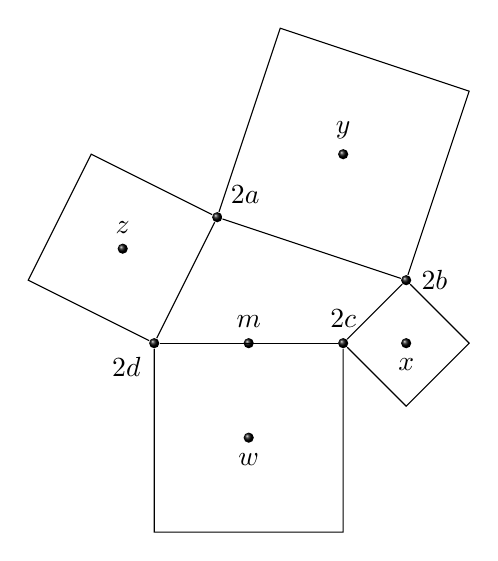
\begin{tikzpicture}
\begin{scope}[scale=0.4]
    %vertices
    \node[ball, label={above right:$2a$}] (A) at (-1,3) {};
    \node[ball, label={right:$2b$}] (B) at (5,1) {};
    \node[ball, label={$2c$}] (C) at (3,-1) {};
    \node[ball, label={below left:$2d$}] (D) at (-3,-1) {};
    %midpoint
    \node[ball, label={above:$m$}] (m) at (0,-1) {};
    %centers
    \node[ball, label={below:$w$}] (w) at (0,-4) {};
    \node[ball, label={below:$x$}] (x) at (5,-1) {};
    \node[ball, label={above:$y$}] (y) at (3,5) {};
    \node[ball, label={above:$z$}] (z) at (-4,2) {};
    %squares
    \draw (A) -- (1,9) -- (7,7) -- (B);
    \draw (D) -- (-7,1) -- (-5,5) -- (A);
    \draw (B) -- (7,-1) -- (5,-3) -- (C);
    \draw (C) -- (3,-7) -- (-3,-7) -- (D);
    %quadrilateral 
    \draw (A) to (B);
    \draw (B) to (C);
    \draw (C) to (D);
    \draw (D) to (A);
\end{scope}
\end{tikzpicture}
\end{document}
    \caption{A coloring of a nonagon}
\end{figure}

\par Without loss of generality, let all the border triangles be red. Counting the edges of all red triangles, we see that every edge and diagonal borders one red triangle. By lemma \ref{2.1}, there are $n$ edges and $n-3$ diagonals, for a total of $2n-3$ diagonals. Furthermore, $2n-3$ must be a multiple of $3$, so $2n$ is a multiple of $3$, and so is $n$.
\end{proof}


\section{Problem 3.}
Prove that it is impossible to divide a given segment in halves with the help of a ruler.
\begin{proof}
With only a straight edge, the only possible constructions are drawing lines between points and finding the intersection between two lines. Suppose we have segment $AB$ in projective plane $P$, and we know a construction that finds midpoint $M$. Then the same construction can find midpoint $M'$ for $A'B'$ in projective plane $P'$. However, we can choose an transformation (which preserves segments and lines) $P\rightarrow P'$  that is injective but does not preserve the $M'$ as the midpoint of $A'B'$. Then, this leads to a contradiction, because the construction of the midpoint in the plane $P$ induces a construction in $P'$ which also would have to lead to the midpoint of $A'B'$.
\par An example projection transformation that does not preserve midpoints is as follows. Suppose all points are on a plane, and there is a point $O$ above this plane. Draw the line from $O$ to points on the first plane and mark its projection on its intersection with the second plane, which is not parallel to the first.

\begin{figure}[ht]
    \centering
    \documentclass{standalone}
\usepackage{tikz}
%------------tikz Setup------------

\tikzstyle{ball} = [circle,shading=ball, ball color=black,
    minimum size=1mm,inner sep=1.3pt]
\tikzstyle{miniball} = [circle,shading=ball, ball color=black,
    minimum size=1mm,inner sep=0.5pt]
\tikzstyle{mminiball} = [circle,shading=ball, ball color=black,
    minimum size=0.6mm,inner sep=0.1pt]
\usetikzlibrary{arrows.meta}
\usetikzlibrary{angles, quotes}
\tikzset{>={Latex[length=2mm,width=1.5mm]}}
\tikzset{->-/.style={decoration={markings, mark=at position #1 with
  {\arrow{>}}},postaction={decorate}}}
\usetikzlibrary{decorations.pathmorphing}
\usetikzlibrary{decorations.pathreplacing}
\usetikzlibrary{arrows.meta,calc}
\usetikzlibrary{bending}
\usetikzlibrary{decorations.markings,shapes.geometric}
\tikzset{->-/.style={decoration={markings, mark=at position #1 with
  {\arrow{>}}},postaction={decorate}}}
\tikzset{-|-/.style={decoration={markings, mark=at position #1 with
  {\arrow{stealth}}},postaction={decorate}}}
\tikzset{movearrow/.style 2 args ={
        decoration={markings,
    mark= at position {#1} with {\arrow{#2}} ,
        },
        postaction={decorate}
    }
}


\begin{document}
\begin{tikzpicture}
\begin{scope}[scale=2.3]
    \node[ball, label={above:$O$}] (o) at (0,1) {};
    \node[ball] (1) at (-2,0) {};
    \node[ball] (2) at (2,0) {};
    \node[ball] (4) at (-1.5,-0.5) {};
    \node[ball] (3) at (2.5,-0.5) {};
    \draw[dashed] (1) to (2);
    \draw[dashed] (2) to (3);
    \draw[dashed] (3) to (4);
    \draw[dashed] (1) to (4);
    \node[ball] (1a) at (-2,0) {};
    \node[ball] (2a) at (2,-1.5) {};
    \node[ball] (4a) at (-1.5,-0.5) {};
    \node[ball] (3a) at (2.5,-2) {};
    \draw[dashed] (1a) to (2a);
    \draw[dashed] (2a) to (3a);
    \draw[dashed] (3a) to (4a);
    \draw[dashed] (1a) to (4a);
    \node[ball, label={above left:$A$}] (A) at (-0.5,-0.25) {};
    \node[ball, label={above right:$B$}] (B) at (0.5, -0.25) {};
    \node[ball, label={above right:$M$}] (M) at (0, -0.25) {};
    \node[ball, label={left:$A'$}] (A') at (-0.65,-0.65) {};
    \node[ball, label={below right:$B'$}] (B') at (0.93, -1.25) {};
    \node[ball, label={below right:$M'$}] (M') at (0, -0.9) {};
    \draw (A) to (B);
    \draw (A') to (B');
    \draw (o) to (A');
    \draw (o) to (B');
    \draw (o) to (M');
\end{scope}
\end{tikzpicture}
\end{document}
    \caption{Example as described above}
\end{figure}

\end{proof}
\end{document}
